\newpage
\section{Implementation Details}\label{app:imp_details}
% \subsection{Dataset Details}
\begin{table}[H]
\caption{Detailed description of 24 instruction induction tasks proposed in \citet{honovich2022instruction}. For convenience, the original table from \cite{honovich2022instruction} is duplicated here.}
\small
\centering
\begin{tabular}{@{}p{0.12\textwidth}@{}p{0.175\textwidth}@{}p{0.375\textwidth}p{0.300\textwidth}@{}}
\toprule
\textbf{Category}                           & \textbf{Task}           & \textbf{Instruction}                                             & \textbf{Demonstration} \\
\midrule
\textit{Spelling} & First Letter & Extract the first letter of the input word. & cat $\rightarrow$  c \\
\cmidrule{2-4}
 & Second Letter & Extract the second letter of the input word. & cat $\rightarrow$  a \\
\cmidrule{2-4}
 & List Letters & Break the input word into letters, separated by spaces. & cat $\rightarrow$  c a t\\
\cmidrule{2-4}
& Starting With & Extract the words starting with a given letter from the input sentence. & The man whose car I hit last week sued me. [m] $\rightarrow$  man, me \\
\midrule
\textit{Morpho-}

\textit{syntax} & Pluralization  & Convert the input word to its plural form.                   & cat $\rightarrow$  cats \\
\cmidrule{2-4} 
                                   & Passivization  & Write the input sentence in passive form.             &
The artist introduced the scientist. $\rightarrow$  The scientist was introduced by the artist. \\
\midrule
\textit{Syntax}                             & Negation       & Negate the input sentence.   & Time is finite $\rightarrow$  Time is not finite. \\
\midrule
\textit{Lexical} 

\textit{Semantics} & Antonyms       & Write a word that means the opposite of the input word. & won $\rightarrow$ lost \\
\cmidrule{2-4}
                                   & Synonyms       & Write a word with a similar meaning to the input word.  & alleged $\rightarrow$  supposed\\
\cmidrule{2-4}
                                   & Membership    & Write all the animals that appear in the given list.    & cat, helicopter, cook, whale, frog, lion $\rightarrow$  frog, cat, lion, whale \\
\midrule
\textit{Phonetics}                          & Rhymes         & Write a word that rhymes with the input word.           & sing $\rightarrow$  ring \\
\midrule
\textit{Knowledge}                    & Larger Animal  & Write the larger of the two given animals.              & koala, snail $\rightarrow$  koala\\
\midrule
\textit{Semantics} & Cause Selection & Find which of the two given cause and effect sentences is the cause. & Sentence 1: The soda went flat. Sentence 2: The bottle was left open. $\rightarrow$  The bottle was left open.\\
\cmidrule{2-4}
& Common

Concept & Find a common characteristic for the given objects. & guitars, pendulums, neutrinos $\rightarrow$  involve oscillations.\\
\midrule
\textit{Style} & Formality & Rephrase the sentence in formal language. & Please call once you get there $\rightarrow$  Please call upon your arrival.\\
\midrule
\textit{Numerical}         & Sum            & Sum the two given numbers.   & 22 10 $\rightarrow$  32 \\
\cmidrule{2-4}
                                   & Difference     & Subtract the second number from the first.  & 32 22 $\rightarrow$  10 \\
\cmidrule{2-4}
                                   & Number to Word & Write the number in English words.  & 26 $\rightarrow$  twenty-six \\
\midrule
\textit{Multi-}

\textit{lingual} & Translation    & Translate the word into German / Spanish / French.    & game $\rightarrow$  juego\\
\midrule
\textit{GLUE} & Sentiment 

Analysis & Determine whether a movie review is positive or negative. & The film is small in scope, yet perfectly formed. $\rightarrow$  positive \\
\cmidrule{2-4}
& Sentence 

Similarity & Rate the semantic similarity of two input sentences on a scale of 0 - definitely not to 5 - perfectly. & Sentence 1: A man is smoking. Sentence 2: A man is skating. $\rightarrow$  0 - definitely not \\
\cmidrule{2-4}
& Word in Context & Determine whether an input word has the same meaning in the two input sentences. & Sentence 1: Approach a task. Sentence 2: To approach the city. Word: approach  $\rightarrow$  not the same \\
\bottomrule
\\
\end{tabular}
\label{tab:instruct_tasks_original}
\end{table}


\begin{table}[H]
\caption{Detailed description of BIG-Bench Instruction Induction (BBII), a clean and tractable subset of 21 tasks that have a clear human written instruction that can be applied to all examples in the dataset.}
\label{table:bbii_desc}
\small
\centering
\begin{tabular}{m{2.5cm}m{5.5cm}m{5cm}}
\toprule
\textbf{Name} & \textbf{Description} & \textbf{Keywords} \\
\midrule
causal judgment & Answer questions about causal attribution & causal reasoning, common sense, multiple choice, reading comprehension, social reasoning \\
\midrule
disambiguation qa & Clarify the meaning of sentences with ambiguous pronouns & common sense, gender bias, many-shot, multiple choice \\
\midrule
dyck languages &  Correctly close a Dyck-n word & algebra, arithmetic, logical reasoning, multiple choice \\
\midrule
epistemic reasoning & Determine whether one sentence entails the next & common sense, logical reasoning, multiple choice, social reasoning, theory of mind \\
\midrule
gender inclusive sentences german & Given a German language sentence that does not use gender-inclusive forms, transform it to gender-inclusive forms & free response, grammar, inclusion, non-English, paraphrase \\
\midrule
implicatures & Predict whether Speaker 2's answer to Speaker 1 counts as a yes or as a no & contextual question-answering, multiple choice, reading comprehension, social reasoning, theory of mind \\
\midrule
linguistics puzzles & Solve Rosetta Stone-style linguistics puzzles & free response, human-like behavior, linguistics, logical reasoning, reading comprehension \\
\midrule
logical fallacy detection & Detect informal and formal logical fallacies & logical reasoning, multiple choice \\
\midrule
movie recommendation & Recommend movies similar to the given list of movies & emotional intelligence, multiple choice \\
\midrule
navigate & Given a series of navigation instructions, determine whether one would end up back at the starting point & arithmetic, logical reasoning, mathematics, multiple choice\\
\midrule
object counting & Questions that involve enumerating objects of different types and asking the model to count them & free response, logical reasoning \\
\midrule
operators & Given a mathematical operator definition in natural language, apply it & free response, mathematics, numerical response \\
\midrule
presuppositions as nli & Determine whether the first sentence entails or contradicts the second & common sense, logical reasoning, multiple choice \\
\midrule
question selection & Given a short answer along with its context, select the most appropriate question which to the given short answer & multiple choice, paraphrase, reading comprehension, summarization \\
\midrule
ruin names & Select the humorous edit that 'ruins' the input movie or musical artist name &    emotional understanding, multiple choice \\
\midrule
snarks & Determine which of two sentences is sarcastic & emotional understanding, humor, multiple choice \\
\midrule
sports understanding & Determine whether an artificially constructed sentence relating to sports is plausible or implausible & common sense, context-free question answering, domain specific, multiple choice \\
\midrule
tense & Modify the tense of a given sentence & free response, paraphrase, syntax \\
\midrule
winowhy & Evaluate the reasoning in answering Winograd Schema Challenge questions & causal reasoning, common sense, multiple choice, social reasoning \\
\midrule
word sorting & Sort a list of words & algorithms, free response \\
\midrule
word unscrambling & Unscramble the given letters to form an English word & free response, implicit reasoning, tokenization \\
\bottomrule
\end{tabular}
\end{table}


\clearpage
\newpage
\subsection{BIG-Bench Instruction Induction (BBII) Selection Process}
\textbf{Step 1}: BIG-Bench contains a large number of evaluation tasks with different level of quality. For example, some of the tasks only have the minimum number of examples needed to qualify for submission, while other tasks may lack an appropriate human baselines. Therefore, we follow \citet{suzgun2022challenging} to get a clean and tractable subset based on the following criteria.
\begin{table}[H]
\vspace{-0.06in}
\caption{Filtering criteria to used to create the BIG-Bench Instruction Induction (BBII) subset.}
\label{table:bbii_filtering}
\vspace{-0.08in}
\small
\centering
\begin{tabular}{m{1cm}m{12cm}}
\toprule
\textbf{\# Tasks} & \textbf{Criteria} \\
\midrule
212 & All BIG-Bench tasks \\
170 & All JSON tasks \\
127 & After filtering out tasks with more than one sub-task \\
74 & After filtering out tasks with fewer than 150 examples \\
67 & After filtering out tasks without human-rater baselines \\
57 & After filtering out tasks that do not use multiple-choice or exact match as the evaluation metric \\
\bottomrule
\end{tabular}
\vspace{-0.1in}
\end{table}

\textbf{Criteria: JSON Tasks.}\\
Discarded tasks: abstraction and reasoning corpus, bbq lite, bias from probabilities, boolean expressions, com2sense, context definition alignment, convinceme, coqa conversational question answering, cycled letters, diverse social bias, dynamic counting, factuality of summary, forecasting subquestions, gender sensitivity chinese, gender sensitivity english, high low game, long context integration, multistep arithmetic, muslim violence bias, program synthesis, protein interacting sites, python programming challenge, question answer creation, roots optimization and games, self awareness, self evaluation courtroom, self evaluation tutoring, simple arithmetic, spelling bee, squad shifts, subject verb agreement, sudoku, taboo, talkdown, text navigation game, training on test set, truthful qa, twenty questions, unqover, web of lies, word problems on sets and graphs, yes no black white.

\textbf{Criteria: Tasks without sub-task.}\\
Discarded tasks: abstract narrative understanding, arithmetic, authorship verification, bbq lite json, cause and effect, chess state tracking, cifar10 classification, color, conceptual combinations, conlang translation, cs algorithms, elementary math qa, fact checker, gem, goal step wikihow, hhh alignment, indic cause and effect, intersect geometry, kanji ascii, key value maps, language games, linguistic mappings, list functions, logical deduction, metaphor understanding, minute mysteries qa, modified arithmetic, mult data wrangling, multiemo, natural instructions, periodic elements, physics, real or fake text, simp turing concept, simple arithmetic json subtasks, simple ethical questions, strange stories, symbol interpretation, tracking shuffled objects, undo permutation, unit conversion, unit interpretation, unnatural in context learning.

\textbf{Criteria: The task includes at least 150 examples with input-output pairs.}\\
Discarded tasks: analytic entailment, auto debugging, code line description, codenames, common morpheme, crash blossom, crass ai, cryobiology spanish, dark humor detection, emoji movie, emojis emotion prediction, empirical judgments, english proverbs, english russian proverbs, entailed polarity, entailed polarity hindi, evaluating information essentiality, figure of speech detection, general knowledge, gre reading comprehension, human organs senses, identify math theorems, identify odd metaphor, implicit relations, international phonetic alphabet nli, irony identification, known unknowns, logical args, logical sequence, mathematical induction, misconceptions russian, nonsense words grammar, novel concepts, odd one out, penguins in a table, persian idioms, phrase relatedness, physical intuition, physics questions, repeat copy logic, rephrase, riddle sense, scientific press release, sentence ambiguity, similarities abstraction, simple arithmetic json, simple arithmetic json multiple choice, simple arithmetic multiple targets json, simple text editing, sufficient information, suicide risk, swedish to german proverbs, what is the tao.

\textbf{Criteria: The task contains reported (average) human-rater or random performance.}\\
Discarded tasks: contextual parametric knowledge conflicts, hinglish toxicity, medical questions russian, parsinlu qa, swahili english proverbs, tellmewhy, which wiki edit.

\textbf{Criteria: The task is classification or uses exact match as the evaluation metric.}\\
Discarded tasks: auto categorization, few shot nlg, hindi question answering, international phonetic alphabet transliterate, polish sequence labeling, qa wikidata, semantic parsing in context sparc, semantic parsing spider, social support, topical chat.

\clearpage
\newpage
\textbf{Step 2}: We do a manual inspection to divide the remaining tasks to the following three categories. In particular, Big-Bench Instruction Induction (BBII) subset is the subet we used to evaluate APE in Section \ref{sec:bigbench}.

\begin{itemize}
    \item \textbf{BBII Subset}: A subset of Big Bench Tasks that satisfy the instruction induction format: each example in the dataset can be expressed as a question-answer pair, all examples focus on the same question that can be clearly described by a human instruction, and there is a human instruction available in the task JSON file.
    \item \textbf{Invalid Format}: Tasks that do not match the instruction induction format: each example in the dataset asks a different question, or clear human instruction is not available. 
    \item \textbf{Out of Scope}: Tasks that are outside the scope of this work: not solvable by authors within 60 minutes, or requires specialized knowledge. 
\end{itemize}

\begin{table}[H]
\caption{Filtering criteria to used to create the BIG-Bench Instruction Induction (BBII) subset.}
\label{table:bbii_categorize}
\small
\centering
\begin{tabular}{m{2cm}m{1cm}m{10cm}}
\toprule
\textbf{\# Category} & \textbf{\# Tasks} & \textbf{Tasks Names} \\
\midrule
BBII Subset & 21 & causal judgment, disambiguation qa, dyck language, epistemic reasoning, gender inclusive sentences german, implicatures, linguistics puzzles, logical fallacy detection, movie recommendation, navigate, object counting, operators, presuppositions as nli, question selection, ruin names, snarks, sports understanding, tense, winowhy, word sorting, word unscrambling.\\
\midrule
Invalid Format & 21 & anachronisms, analogical similarity, bridging anaphora resolution barqa, data understanding, disfl qa, fantasy reasoning, formal fallacies syllogisms negation, hindu knowledge, hyperbaton, intent recognition, logic grid puzzle, paragraph segmentation, play dialog same or different, reasoning about colored objects, salient translation error detection, social iqa, strategyqa, temporal sequences, timedial, understanding fables, vitaminc fact verification.\\
\midrule
Out of Scope & 13 &ascii word recognition, checkmate in one, chinese remainder theorem, cryptonite, discourse marker prediction, geometric shapes, kannada, language identification, matrixshapes, mnist ascii, moral permissibility, movie dialog same or different, parsinlu reading comprehension.\\
\bottomrule
\end{tabular}
\end{table}


% \hline \text { \# Tasks } & \text { Criteria } \\
% \hline \frac{209}{187} & \text { All BIG-Bench tasks } \\
% 130 & \text { - After filtering out tasks with more than three subtasks } \\
% 85 & \text { - After filtering out tasks with fewer than } 103 \text { examples ( } 3 \text { for few-shot, } 100 \text { for evaluation) } \\
% 78 & \text { - After filtering out tasks without human-rater baselines } \\
% \hline \frac{78}{36} & \text { Clean multiple-choice or exact match tasks } \\
% 23 & \text { - After filtering out tasks in which the best reported model beats average reported human-rater score } \\
% \hline 23 & \text { Remaining tasks = BIG-Bench Hard (BBH) } \\

\clearpage
\newpage
\workshopexclude{
\begin{table}[H]
\caption{Raw templates used for model prompting in our experiments}
\label{table:raw_templates}
\centering
\begin{tabular}{m{3.2cm}m{\textwidth-4cm}}
\toprule
\textbf{Usage} & \textbf{Template} \\
\midrule
Zero-shot Evaluation & 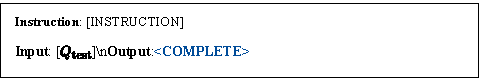
\includegraphics[scale=1.25]{figures/appendix/zeroshot_template.pdf} \\
\midrule
Few-shot Evaluation & 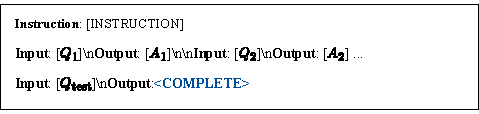
\includegraphics[scale=1.25]{figures/appendix/fewshot_template.pdf}\\
\midrule
{Forward Generation} & 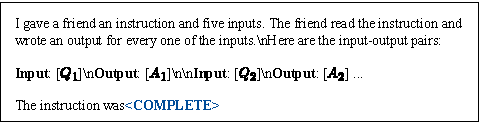
\includegraphics[scale=1.25]{figures/appendix/forward_template.pdf}\\
\midrule
Reverse Generation 1 & 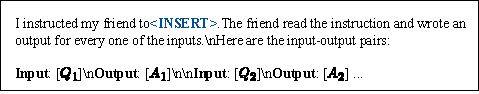
\includegraphics[scale=1.25]{figures/appendix/insert_template.pdf}\\
\midrule
Reverse Generation 2 & 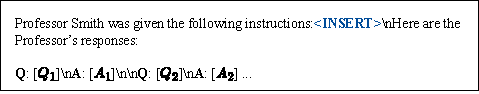
\includegraphics[scale=1.25]{figures/appendix/truthful_template.pdf}\\
\midrule
Resample Instruction & 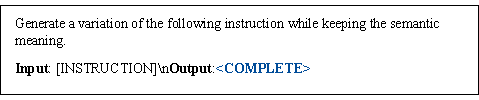
\includegraphics[scale=1.25]{figures/appendix/iterative_template.pdf} \\
\midrule
Zero-shot-CoT & 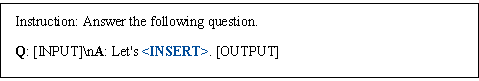
\includegraphics[scale=1.25]{figures/appendix/cot_template.pdf} \\
\bottomrule
\end{tabular}
\end{table}
}


\workshoponly{
\begin{table}[H]
\caption{Raw templates used for model prompting in our experiments}
\label{table:raw_templates}
\centering
\begin{tabular}{m{3.2cm}m{10cm}}
\toprule
\textbf{Usage} & \textbf{Template} \\
\midrule
Zero-shot Evaluation & 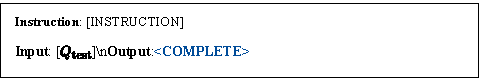
\includegraphics[scale=1.25]{figures/appendix/zeroshot_template.pdf} \\
\midrule
Few-shot Evaluation & 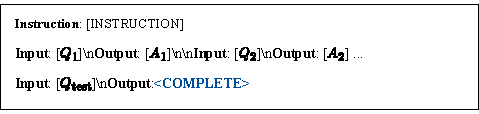
\includegraphics[scale=1.25]{figures/appendix/fewshot_template.pdf}\\
\midrule
{Forward Generation} & 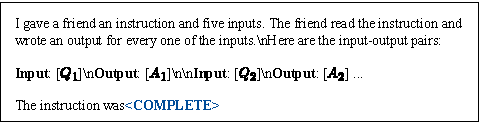
\includegraphics[scale=1.25]{figures/appendix/forward_template.pdf}\\
\midrule
Reverse Generation 1 & 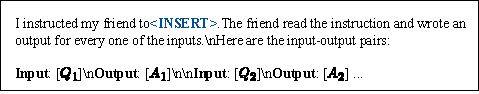
\includegraphics[scale=1.25]{figures/appendix/insert_template.pdf}\\
\midrule
Reverse Generation 2 & 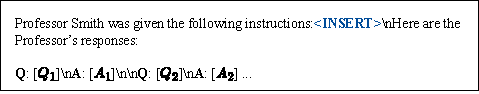
\includegraphics[scale=1.25]{figures/appendix/truthful_template.pdf}\\
\midrule
Resample Instruction & 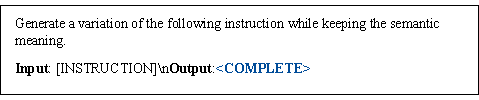
\includegraphics[scale=1.25]{figures/appendix/iterative_template.pdf} \\
\bottomrule
\end{tabular}
\end{table}
}